%%%%%%%%%%%%%%%%%%%%%%%%%%%%%%%%%%%%%%%%%%%%%%%%%%%%%%%%%%%%%%%%%%% 
%                                                                 %
%                             Animation                           %
%                                                                 %
%%%%%%%%%%%%%%%%%%%%%%%%%%%%%%%%%%%%%%%%%%%%%%%%%%%%%%%%%%%%%%%%%%% 
 
\chapter{ANIMATION}
\label{chapter:animation}

Jumping is the acceleration of a character's center of mass upward.  This motion can be divided into several stages.  First is the lead-up or wind-up stage in which the character flexes or gathers momentum to perform the jump.  This takes the form of a slight crouch (TODO reference cat jumping paper or the background .  should this be in background?) which prepares the character to exert the necessary force against the ground.  

Next comes the take-off stage.  The character pushes against the floor with their feet, accelerating their center of mass to break contact with the floor.  

\section{Setup and Inputs}
%TODO should this just be in the animation section?
The character in our system consists of a mesh, a skeleton, and a controller which has itself several sub-components.  First we constructed a mesh, a 3D visual representation of our character.  Our mesh is a simple, blocky humanoid, lacking arms in order to focus more heavily on the lower body motion of the figure.  A more complex human character, or even a humanoid non-human character could be substituted.  This mesh consists of vertices, which each have a position as well as other information not relevant to our simulation such as normal and texture coordinate, which are used by \unity for displaying the mesh.  This mesh can also be referred to as a character model, but in the context of this simulation we will refer to it as the mesh.  Three vertices form a triangular face, though these are often created as quadrilaterals by the artist as the topology of the model can be simpler to work with due to the grid patterns formed as compared to triangular meshes.  In the case of quad meshes, the mesh is often treated as a triangle mesh by the game engine or renderer, with each quad producing two triangles.

Our mesh was created using \maya, positioning the vertices in groups or individually, using several rectangular prisms as a base.  Using the edge loop tool, more vertices were inserted, with loops of edges circling the torso and legs to produce the final shape.  This mesh was then rigged, meaning a skeleton was added.  As described in further detail in \ref{subsection:skel_joints}, joints were positioned individually relative to the mesh, attempting to mimic the positioning of joints in the human skeleton.  The connections were made simply, with each joint acting as a ball and socket joint, meaning that constraints needed to be specified at a later stage to facilitate hinge joints such as the knee and ankle and that complex, multi-boned structures as found in the foot and shin were simplified to a single bone connecting two joints.  The hierarchy of joints for the skeleton was rooted at the pelvis with three children: one leading to the upper body and one to each hip.  From there a single joint was used for the manipulation of the upper body, with separate joints for each hip, knee, ankle, toe, and heel.  Though there is no movement in the toe, placing a bone for the foot requires an end joint for the bone to connect to.

%TODO how do i talk about this with authority, there isn't really anything to cite there's just youtube videos and it's generally taught as such/discovered via industry
Joints are then associated with the mesh through weight painting, in which each vertex of the mesh is assigned a weight for each joint.  This weight designates if and how much a vertex transforms when a joint is moved.  Each vertex must be assigned a weight for each joint of the model.  Careful weight assignment is highly important as this determines the behavior of the character's ``skin'' when they move, affecting how the mesh twists or bends as well as which parts move with which bones.  The joints may then be used to manipulate the mesh to produce animations, with each keyframe in an animation storing information about each joint instead of each vertex.

\subsection{User Specified Constants}
\label{subsection:user_constants}
% specified constants
% gravity
% air time
% windup time
% error allowance (between calculated skeleton values and desired)
% drag
% jumping policy (not implemented)
% Windup PD k values
% Balance PD k values
% muscle values foreach muscle:
%	k (linear spring constant)
%	anchor joints (for our simulation, 2)
% 	center joint
%   [0,1] scale to indicate muscle anchor position (0 is closer to center joint, 1 is closer to end joint)
%   bone width
% calculated values
Within the controller there are a number of constants the user can specify, outside of the character itself.  These specify constants for the simulation environment as well as some constants describing the animation to be produced.  Our only environmental constant is gravity, which we specify as -10 $\frac{m}{s^2}$, where the negative indicates the downward direction.  Other constants include the air time, windup time, error allowance, and constants for the PID controllers.

The times indicate how much time the character is expected to spend in the air and winding up for the jump.  Air time in our case consists of the portion of the animation where the character's feet are not in contact with the ground plane.  Windup time refers to the time in which the character has their feet on the ground and is in the process of accelerating their mass upwards as the initial takeoff portion of the jump.  A long windup time gives a very slow, exaggerated jumping motion while a short windup gives a very rapid, clipped motion.  While we allow the user to specify any time for both air and windup, in practice there is a limited range of values that are possible for the character.

%TODO example windup times with our chosen values

\subsection{Skeleton, Joints, and Muscles}
\label{subsection:skel_joints}
For the purposes of animation, a joint is an object with an associated position, associated transformation, a parent joint, and some number of child joints.  In the case of the root, the parent joint is absent and in the case of the end joints such as tips of the fingers there are no child joints.  Each child joint is connected to the parent by a rigid bone, which protrudes from the parent at a given resting angle.  These joints are structured in a tree, as the parent and child joints imply, with the root of the tree at the pelvis.  This tree serves as a hierarchy for transformations.

Joints are associated with a set of vertices from the mesh to be animated.  Each of these may be associated with multiple joints, and are assigned a weight for each joint which acts as a scale factor for the transformations performed on the vertex.  When a joint is transformed, the transformation is propagated to the children, with the parent as the origin of the child node's coordinate system.


%%%%%%%%%%%%%%%%%%%%%%%%%%%%%%%%%%%%%%%%%%%%%%%
%               Torque Method                 %
%%%%%%%%%%%%%%%%%%%%%%%%%%%%%%%%%%%%%%%%%%%%%%%
\section{Torque-based simulation}
One method of simulation we attempted used springs placed along the length of each limbs to produce a torque on the joints of the character.  This method failed for unknown reasons.  Torques on the joints results from the force of the muscle pulling a bone to rotate about the joint, resulting in a complex system of motion with each bone rotating around the joints.  These rotations combine to move the body in a direction, allowing a character's control to be centered around degree and timing of muscle activation. \cite{muscle_based_bipeds}  In our case, we take the muscle as fully activated, which means that it has a spring constant defining the strength of the muscle.  This muscle is then stretched to produce the desired torque by bending the affected limb.  The restoring force of the spring-muscles produce torques which are used to calculate angular momentum, and from that linear momentum.  

\subsection{Path Estimation}

\begin{figure}[ht]
	\centering
	\begin{tikzpicture}[node distance=1cm and 1cm, auto]
% Path Estimate Phase
	%	Path Estimate Stage
    \node [stage] (path) {\nodebox{5cm}{Path Estimate \[a = \dfrac{2 (x - x_0 - v_0 t)}{t^2} \]}};
    %	Path Estimate Data
    \node [data, above= of path] (xf) {\nodebox{2cm}{Target Position ($x$)}};
    \node [data, left= of xf] (xi) {\nodebox{2cm}{Initial Position ($x_0$)}};
    \node [data, left= of xi](t) {\nodebox{2cm}{Time ($t$)}};
    \node [data, right= of xf] (vi) {\nodebox{2cm}{Initial Velocity ($v_0$)}};
    \node [data, below= of path] (accel) {\nodebox{3cm}{Target Acceleration ($a$)}};
    
    \path [line] (xi) |- (path);
    \path [line] (xf) -- (path);
    \path [line] (t) |- (path);
    \path [line] (vi) |- (path);
    \path [line] (path) -- (accel);
\end{tikzpicture}
	\caption[Diagram of path estimation algorithm]{Diagram of the path estimation step.}
	\label{fig:pathEstimate}
\end{figure}

\begin{figure}[ht]
	\label{fig:pathExample}
	\caption[Example of estimated path]{Example of a path estimation.}
\end{figure}
Before calculations relating to the model's skeleton are performed, an initial estimate of the jump path is performed.  The estimate uses a simple forward kinematic calculation to determine the force required to move an object through the air from the initial position of the model, denoted as $x_0$ in Figure \ref{fig:pathEstimate}, to a final position, denoted as $x$.  To facilitate a character jumping while moving, the path estimate takes into account the initial velocity $v_0$.

The user specifies a desired time ($t$), which indicates the time the character will spend airborne during the animation, i.e. the time between when the character's feet break contact with the ground and when they regain contact with the ground.  This is useful as the desired animation can be more easily adjusted to fit a desired time as an in-game animation or to fit a particular storyboard for an animated film sequence.

\subsection{Windup}
From this force, the acceleration can be determined using $F=ma$ from classical mechanics.  This assumes the character is a rigid body with negligible air resistance acted upon by gravity of $10\frac{m}{s}$.  The mass is calculated as the summed total of the distributed masses assigned to the character's limbs, which are summed to produce a total mass for the character.

Proportional derivative control is used to produce the windup motion once the initial path estimate is calculated.  The error function $E_{all}$ calculates error from the desired force $E_{force}$ as well as the balance $E_{balance}$.

Once computed, error is compared to a threshold ($\epsilon$).  If the error is below the threshold, the skeleton is considered bent to the proper position for windup and the system proceeds to the thrust phase in which the character unbends.  If the value is above the threshold, a new position for the hip is calculated using proportional-derivative control, where the new position for the iteration of the controller, $u(i)$, is calculated as \[u(i) = k_p E_{all}(i - 1) + k_d(E_{all}(i-1) - E_{all}(i-2))\] where $i$ is the iteration, and $k_p$ and $k_d$ are weights which determine the rate of change. This new hip position is given to an inverse kinematics component to calculate the positions of the remaining leg joints, assuming the feet should remain in the same position.  These new joint positions and angles are then passed back to the PD controller to re-calculate the center of mass as well as the new force and balance errors for the next iteration.

\begin{figure}[ht]
	\centering
	\resizebox{\textwidth}{!}{
		\begin{tikzpicture}[node distance = 0.5cm, auto]
% Bend Phase
    % before controller, need to calculate the desired 
    % place nodes
    \node [data, below of=path] (accel) {\nodebox{2.5cm}{Target Acceleration ($a$)}};
	\node [data, left=of accel] (mass) {\nodebox{3.5cm}{Body Mass assigned to each limb ($\left\lbrace m_0, \ldots, m_n\right\rbrace$)}};
    \node [stage, below= of accel] (forceCalc) {\nodebox{6cm}{Calculate desired force $F_{target} = \displaystyle\sum_{j=0}^n {m_j} a$}};
    % connecting lines
    \path [line] (accel) -- (forceCalc);
    \path [line] (mass) |- (forceCalc);
    % ----------------
	
    % PD controller
    % place nodes
    \node [substage, below=5cm of forceCalc] (bendErr) {Calculate error from desired force magnitude ($E_{force}$)};
    \node [substage, left=2.5cm of bendErr] (bendBal) {Calculate balance error ($E_{balance}$)};
    \node [substage, above=1cm of bendBal] (comCalc) {\nodebox{5cm}{Calculate Center of Mass \[C_{mass} = \displaystyle\sum_{\forall m} m \cdot position(m)\]}};
    \node [data, below left=1cm and -2cm of bendErr] (bendErrAll) {\nodebox{4cm}{$E_{all} = E_{force} + E_{balance}$}};
    \node [decision, below=0.5cm of bendErrAll] (bendPDTest) {$E_{all} \overset{?}{\le} \epsilon$};
    \node [substage, left=1cm of bendPDTest] (bendPDEq) {Set new hip position based on $u(i) = k_p E_{all}(i-1) + k_d \left(E_{all}(i-1) - E_{all}(i-2)\right)$};
    \node [stage, label={[shift={(-0.5cm, 2cm)}, rotate=90]180:\LARGE PD Controller}, fit=(comCalc) (bendErr) (bendBal) (bendErrAll) (bendPDEq) (bendPDTest)] (bendPD) {};
    \node [data, below=2cm of bendPDTest] (bentSkel) {\nodebox{3cm}{Skeleton in bent position ($\theta_{x} \forall x \in J_m$)}};
    \node [data, below=1cm of bendPDEq] (bendPDConst) {
    \nodebox{4cm}{Proportional and Derivative weights ($k_p, k_d$)}};
    % connecting lines
	\path [line] (forceCalc) -- (bendErr);
	\path [line] (comCalc) -- (bendBal);
	\path [line] (bendErr) |- (bendErrAll);
    \path [line] (bendBal) |- (bendErrAll);
    \path [line] (bendErrAll) -- (bendPDTest);
    \path [line] (bendPDTest) -- (bendPDEq);
    \path [line] (bendPDTest) -- (bentSkel);
    \path [line] (bendPDConst) -- (bendPDEq);
    % ----------------
    
    % CoM inputs
    % place nodes
    \node [data, above =2cm of comCalc] (skeleton) {\nodebox{2.5cm}{Model with skeleton attached ($J = \left\lbrace j_0, \ldots, j_n \right\rbrace$, contains at least a pelvis and both left and right hips, knees, ankles, heels, and toes)}}; 
    \node [data, left=1cm of skeleton] (mjoints){\nodebox{3cm}{Muscled joints ($J_m = \lbrace$ $j_{pelvis}$, $j_{Lhip}$, $j_{Rhip}$, $j_{Lknee}$, $j_{Rknee}$, $j_{Lankle}$, $j_{Rankle}$, $j_{Lheel}$, $j_{Rheel}$, $j_{Ltoe}$, $j_{Rtoe}$ $\rbrace$}};
    \node [data, left=1cm of mjoints] (muscles) {\nodebox{3cm}{Muscle spring constant for muscled joints ($\left\lbrace k_0, \ldots, k_11\right\rbrace$)}};
	\node [data, left=1cm of muscles] (jconst) {\nodebox{2cm}{Rotation constraints for joints ($\theta_{min}, \theta_{max}$ $\forall j \in J_{muscled}$)}};
	
	% connecting lines
	\path [line] (skeleton) -- (comCalc);
	\path [line] (mjoints) -- ++(0cm, -3.4cm) -| (comCalc);
	\path [line] (muscles) -- ++(0cm, -3.5cm) -| (comCalc);
	\path [line] (jconst) -- ++(0cm, -3.6cm) -| (comCalc);
	% ----------------	
	
	% IK solver side stage
	% place nodes
	\node [data, left=3cmof bendPDEq] (IKCurJoint) {\nodebox{4cm}{$R = position(j)$ $\forall j \in J_{ik} \subseteq J$ starting with the root (hip joint).}};
	\node [data, left=1cm of IKCurJoint] (IKTargetPos) {\nodebox{4cm}{Target position for joint, in this case keeping $E$ in it's original position ($D$).}};
	\node [data, left=1cm of IKTargetPos] (IKEndJoint) {\nodebox{2cm}{Joint to move to target ($E$).}};
	\node [data, above=1cm of IKEndJoint] (IKRE) {\nodebox{3cm}{Normalized vector $\vec{RE}$}};
	\node [data] (IKRD) at (IKCurJoint |- IKRE) {\nodebox{3cm}{Normalized vector $\vec{RD}$}};
`	\node [substage, above=2cm of IKTargetPos] (IKEq) {$\theta_j = \vec{RD} \times \vec{RE}$.};
	\node [data, above left=1cm of IKEq] (IKItrs) {\nodebox{3cm}{Number of iterations for IK solver ($num_itr$)}};
	\node [data] (IKPartBent) at (IKEq |- comCalc) {\nodebox{2cm}{Bent skeleton reflecting $u(i)$.}};
	\node [stage, label={[shift={(-0.5cm, 1.5cm)}, rotate=90]180:\LARGE IK Solver}, fit=(IKCurJoint) (IKEndJoint) (IKTargetPos) (IKItrs) (IKRD) (IKEq) (IKPartBent)] (bendIK) {Requires joints to be in a single chain.};
    % connecting lines
    \path [line] (bendPDEq) -- (IKCurJoint);
    \path [line] (IKPartBent) -| ++(6cm, -1.6cm) -| (bendErr);
    \path [line] (IKPartBent) -- (comCalc);
    \path [line] (IKCurJoint) -- (IKRD);
    \path [line] (IKEndJoint) -- (IKRE);
    \path [line] (IKTargetPos) |- (IKRD);
    \path [line] (IKTargetPos) |- (IKRE);
    \path [line] (IKRD) |- (IKEq);
    \path [line] (IKRE) |- (IKEq);
    \path [line] (IKEq) -- (IKPartBent);
    \path [line] (IKItrs) |- (IKEq);
    % ----------------
\end{tikzpicture}
	}
	\caption[Diagram of windup phase algorithm]{Algorithm diagram of the windup phase.}
	\label{fig:bendPhase}
	%TODO decision lines need to be labeled
\end{figure}

\begin{table}[ht]
	\centering
	\caption[Table of PD controller constants for windup phase]{Example values for the PD controller constants, showing the sweet spot that we use as well as the effect of going higher or lower (how do we show this effect, show that the steps are too large or too small? time or iterations to finish?).}
	\label{tab:windup_pd_vals}
\end{table}

\subsubsection{Force calculation}
%TODO force calculation should be done with error in net torque instead of error in force as we don't really have a resultant force here and the net force really means nothing
% calculation of the muscle flexion
\begin{figure}[ht]
	\centering
	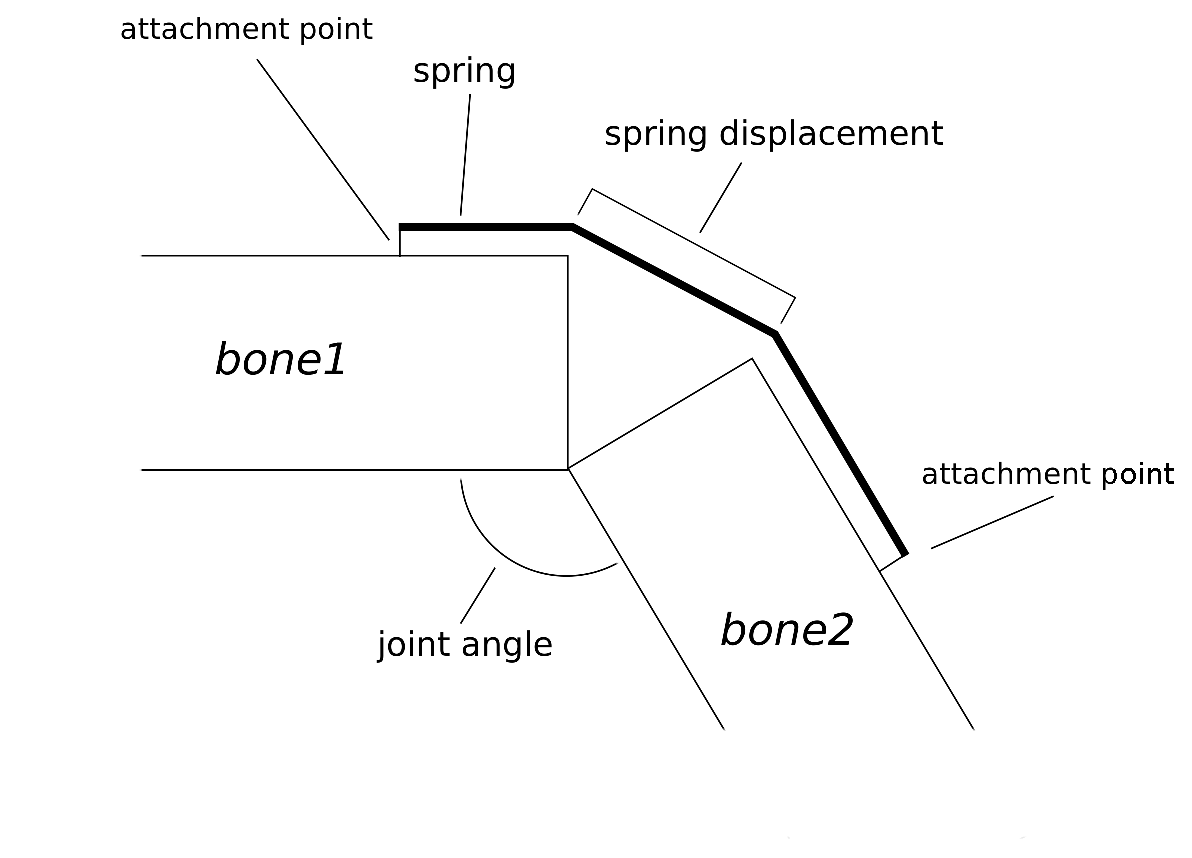
\includegraphics[width=10cm]{images/spring_calc/spring_angle_calc.eps}
	\caption[Diagram of joint force calculation]{Force calculation for a joint.}
	\label{fig:forceCalc}
\end{figure}
Current force is computed by approximating muscles as linear springs attached to two bones and crossing a joint.  The change in spring length is produced by the bend of the joint which opens a space between the rigid bones that the spring must stretch across.  This approximation uses spring constants that simulate a flexed muscle that has been stretched by an amount equal to \[\theta = cos^{-1} \left( \dfrac{2 k^2 r^2}{F^2} - 1 \right)\] which requires a more rigid spring constant.  In this equation, $r$, represents the width of the bone, which is a constant that changes the amount the character must bend to achieve a force.  This acts similarly to the $k$ value, which represents the stiffness of the spring, or a constant for the linear restoring force of the muscle.  
%TODO For our simulations, we used values in the range ().
%TODO values and equation
%TODO tables of values with varied k and varied r and corresponding bend/angle
\begin{table}[ht]
	\centering
	\caption[Table of spring muscle constants]{A table of various values for k and r, demonstrating effect on the model's bend.  TODO Columns of k and r (varied individually), and image of fully bent character resulting from values.}
	\label{tab:variedSpringValues}
\end{table}

At each iteration of the PD controller, current force output of the legs is computed.  An accurate calculation of the force must take into account the torques ($\vec{\tau}$) produced by the muscles on each joint.  We use a simplified version, calculating the magnitudes of the torques which avoids the complexity of implementation and computation.  This is found for a joint j as \[\tau_j = ||\vec{r_j}|| F_j\] where r is the moment arm, the cross product between the vector between the attachment point of muscle and the center of the joint with the direction of the muscle crossing the joint.  Direction of a muscle is in the direction of restoration of the spring (TODO double check this, is this always the value we want, point placed along the spring based on the masses on each end) as used in \cite{muscle_based_bipeds}.
%TODO does this setup effectively result in springs connected in series? No because you can assume that the muscles you don't want to unbend with remain rigid?
%TODO does this give a sort of impulse function as you unbend at the hips and knees, then the ankles?
%TODO this is where the torques come into play, and they're absolutely necessary

\begin{figure}[ht]
	\centering
	\caption[Algorithm diagram for calculation of force error]{Force error calculation}
	\label{fig:forceErr}
\end{figure}

To calculate the error used for PD control, the vector between the two forces is measured, indicating the change required in both direction and magnitude.  As we require the force to act in the direction of acceleration, the main adjustment is the force magnitude.  When instead considering the torque magnitude, the magnitude alone can be considered. (TODO I think I need to be using the torque magnitude instead of a force here).

\subsubsection{Center of Mass and Balance}
%TODO need to standardize usage of joint to anatomical, animation, or something else
The center of mass (CoM) is calculated as the centroid of the character.  More specifically, joint positions are averaged, with a weight assigned to each joint based on the weight of the limb associated.  The CoM must be recalculated with each update to the character's pose as the shift in weight changes the position.

Using the calculated CoM, the balance of the character can be determined by the position of the CoM relative to the supporting polygon of the character.  The supporting polygon is a polygon determined by the points of contact of the character with the ground or other supports which provide a normal force to counteract gravity and other external forces.  During the windup and thrust phases, the character maintains contact with the ground through their feet, with the outer edges of the feet forming two sides of a quad, a line between the two feet at the toes forming a third, and a line between the heels of the character forming the fourth side.  This polygon should be parallel to the ground plane, and is positioned at the bottom of the feet.  If the character's center of mass is over this supporting polygon, the character is balanced.

\begin{figure}[ht]
	\centering
	\caption[Algorithm diagram for calculation of balance error]{Balance error calculation.}
	\label{fig:balanceErr}
\end{figure}

To quantify balance, the vector between the center of the supporting polygon and the position of the CoM is measured.  This vector is then projected into the same plane as the supporting polygon, giving a 2 dimensional error between where the CoM is currently and where it would need to be to be perfectly centered.  The PD controller then attempts to minimize the magnitude of this vector by moving in the proscribed direction while bending to achieve the desired force, constraining the number of solutions possible to provide the desired force.
% does the vertical distance have effect?  you're going to fall over more easily if you're on a stilt as opposed to crouching over your feet as the moment will be (bigger? is that bigger?).  the lever will be more able to move your weight easily

\subsubsection{Inverse Kinematic Solving}
As the skeleton is a hierarchy assumed to be rooted at the hip, a problem arises with applying rotations to joints.  To keep a character's feet rooted to the floor as is expected, positions must be solved for using inverse kinematics.  Given the desired position for the hip, and the desired position of the foot, the joint angles and positions of the knee and ankle are solved for.  Constraints are placed on each joint, limiting the range of motion to an expected range as well as limiting the axes about which each joint can rotate, preventing unnatural directions of motion.  These values are specified per joint and can be edited by the user to simulate varied levels of flexibility or alternate body shapes.

%TODO alternate body with digitigrade, Tauren or whatever from WoW, raptor style...
%TODO Further justification of why choosing this method instead of learning is that this is more user-tunable as opposed to a learning heavy model which doesn't allow as much user tuning

\begin{table}[ht]
	\centering
	\caption[Table of joint constraints]{Joint angle constraint values used for each joint, with accompanying images of expected motion range.}
	\label{tab:jointConstraints}
\end{table}

A solution to the joint positions is found using these constraints, and gradient descent method which works on single-chains of joints.  A single chain of joints is a sequence of joints in which each joint has a single child and a single parent, with one root joint and one leaf joint which lack a parent and child respectively.  Given the hierarchy of joints and a desired position for one of the non-root nodes of the chain, cyclic-coordinate descent (CCD) is used to determine rotations of the joints between the joint in question and the root that will minimize the distance between the joint in question and the desired position.  This algorithm is shown in \ref{alg:ik}.

\begin{algorithm}[ht]
	\centering
	\begin{algorithmic}[H]
		\Function{SingleChainIK}{C, D, E}
		\Repeat
		\ForAll{Joints R between E and the root, starting with the end E}
			\State $\theta_R = \vec{RD} \times \vec{RE}$
		\EndFor
		\Until{\textit{Desired number of iterations performed} or \textbf{E} \textit{is close enough to} \textbf{D}}
		\EndFunction
	\end{algorithmic}
	\caption[Single chain IK algorithm]{Given chain of joints C, move joint E to position D using cyclic coordinate descent (TODO cite CCD references).  This process iteratively moves joint E closer to the location D, concentrating on each joint R in the chain one at a time and solving the geometric problem of minimizing distance between E and D by rotating R.}
	\label{alg:ik}
\end{algorithm}

This approach, while for the specific case of single chains of joints, is simpler to implement than other approaches such as the pseudo-inverse of the Jacobian.  In addition, this approach allows some flexibility, specifically in constraints of the joints.  As each joint is addressed individually instead of the system as a whole, any constraints placed on the joint can easily be accounted for by simply preventing the joint from rotating out of the desired range while the rest of the system continues to move as close as possible to the solution.  One downside is that a halting condition must be determined, through a minimum acceptable distance.  To handle the case where the joint cannot be moved within this minimum distance, a maximum number of iterations must be designated.  In practice, 100 iterations is enough to converge, with as few as 30 working well for our simulation.

\subsection{Thrust and Takeoff}
Upward acceleration is animated by calculating the angular accelerations of the joints given the forces acting upon them and the resulting torques.  Torque is the change in angular momentum over time, allowing for the acceleration to be calculated as the mass can be assumed to be constant: \[\tau = \dfrac{dL}{dt} = m \dfrac{dv_{\theta}}{dt} = m a_{\theta}\] where $\tau$ is the torque of a joint, $L$ is the angular momentum, $m$ is the mass of the limb, which must take into account the mass of the rest of the body which is also moved by the limb, $v_{\theta}$ is the angular velocity and $a_{\theta}$ is the angular acceleration. This results in the below equation for determining angular acceleration. \[a_{\theta} = \dfrac{\tau}{m}\]

Using angular acceleration, the intermediary poses for the model can be determined at each timestep.   For each frame, an explicit Euler integration is performed to determine first angular velocity and finally angle.  As the character continues to extend, a check is made for if the character has yet reached full extension.  At full extension, the character can no longer accelerate in the direction of the jump, and the character breaks contact with the ground to enter the in-air phase.

\subsection{Sampling}
To determine which of numerous possible solutions is the most desirable, we take several samples.  A sample is described by the position of the pelvis joint, the resulting linear momentum, and a vector describing the displacement of the character's center of mass from the center of its support to indicate balance as described above.

Samples were restricted to a box defined by a rectangle around the character's feet with a height reaching the position of the character's pelvis when standing at rest.  Any sample outside of this volume is assumed to put the character off balance.  Samples were then taken at uniformly distributed positions in this region.  The calculated acceleration was projected onto the desired acceleration vector through the dot product, with values greater than or equal to the desired acceleration's magnitude indicating a plausible solution.  These plausible solutions are then ordered by their balance error, calculated as the difference in position between the center of mass and the center of the supporting polygon.  The first result of this list is then chosen as the candidate answer and the pelvis is moved towards this sample.  At each iteration this is repeated until the desired acceleration is achieved.
%To select the minimum sample, the collected data were organized first by the difference between the linear momentum calculated and the desired linear momentum, and the top ten percent were selected.  Ten percent was found empirically to be a good selection of points to select the most balanced from while also retrieving points with very low differences from the desired.

\subsection{Rebalancing}
As the character re-positions its pelvis, the balance must be calculated again and its position accordingly re-adjusted.  To maintain the position of the legs, we use the upper body to achieve balance.  A separate PD controller is used to regulate the rate of movement

%%%%%%%%%%%%%%%%%%%%%%%%%%%%%%%%%%%%%%%
%               Energy                %
%%%%%%%%%%%%%%%%%%%%%%%%%%%%%%%%%%%%%%%
\section{Energy based calculation}
Another way we considered using for simulation was energy based.  We assumed that the energy required to lift the mass of the character and move it the necessary distance is equivalent to the summed elastic potential energies of the leg muscles.  The direction of the velocity is determined by the direction the center of mass is accelerated after the windup phase, and we assume that 

\section{Summary}
\label{subsection:animation_summary}